\documentclass[a4paper,11pt]{article}
\usepackage{fancyhdr}
\usepackage[utf8]{inputenc}
\usepackage{graphicx}
%\setlength{\headheight}{11pt}

\lhead
\rhead
\parskip 1em
\parindent 0em

\begin{document}
\pagestyle{empty}
%-----------------------------------------------------------
\begin{titlepage}

\title{\Huge{Lab report} \\[0.1cm] \Large{Digital Design (EDA322)} \\ [0.4cm] \Large{ \emph{Writing Guidelines}} \\[0.4cm]}
\author{\large{\emph{Group TUE\_PM\_8}} \\[0.2cm] Niklas Gustafsson \\[0.05cm] Oskar Lundström \\[0.1cm]}
\maketitle
\thispagestyle{empty}
\end{titlepage}
\clearpage
%-----------------------------------------------------------
\pagestyle{fancyplain}
\pagenumbering{roman}
\tableofcontents
\clearpage
%%%%%%%%%%%%%%%%
% Introduction
\pagenumbering{arabic}
\setcounter{page}{1}
\section{Introduction}
(max: 1 page)
\\\\
This part will introduce the reader to the report. 

At the beginning, describe what the purpose of this lab report is. Then describe briefly what each section discusses and finally summarize the most important conclusions. 

\newpage
\section{Method}
\subsection{Arithmetic and Logic Unit (ALU)}

When we built our ALU we began by constructing the most basic component, the full-adder. We started by minimizing the boolean expression for the sum and the carry out signals using a Karnaugh diagram. We came to the conclusion that a full-adder should be built like described in the picture below.

\begin{figure}[h!]
  \centering
  
\includegraphics[width=0.5\linewidth]{fulladder.png}
  \caption{A full-adder.}
  \label{fig:etikett}
\end{figure}

You can also build a full-adder using two half-adders and some extra logic. We came to this conclusion by connecting the resulting signal of the first half-adder to the second one along with the carry in signal. After this we just added the extra logic that was needed, which was an OR gate.

\begin{figure}[h!]
  \centering
  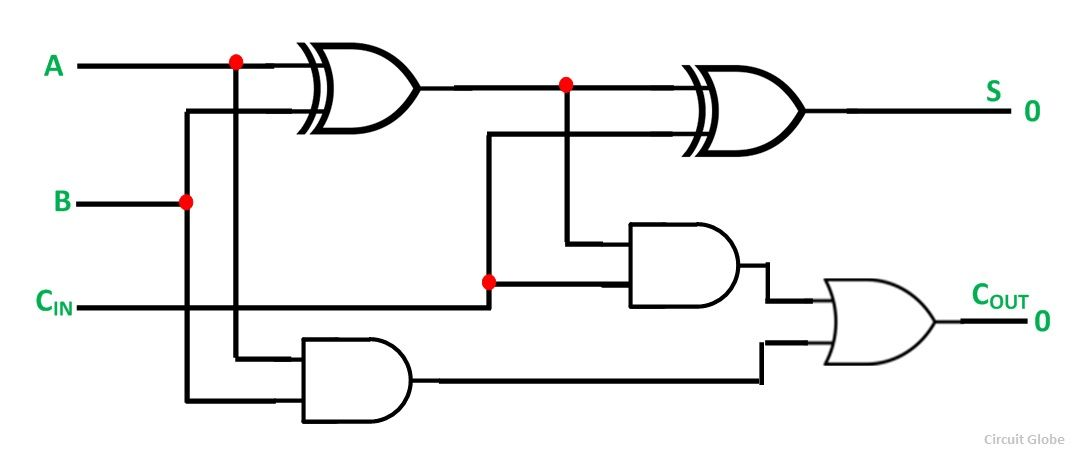
\includegraphics[width=0.5\linewidth]{fulladderfromhalfadder.jpg}
  \caption{A full-adder made from two half-adders.}
  \label{fig:etikett}
\end{figure}

We created an 8-bit ripple carry adder (RCA) by connecting eight full-adders together according to the diagram below. The idea is to simply connect the carry out signal of the first full-adder to the carry in signal of the second one, and so on. The RCA was used in our original design of the ALU but later we replaced it with a carry lookahead adder (CLA).

\begin{figure}[h!]
  \centering
  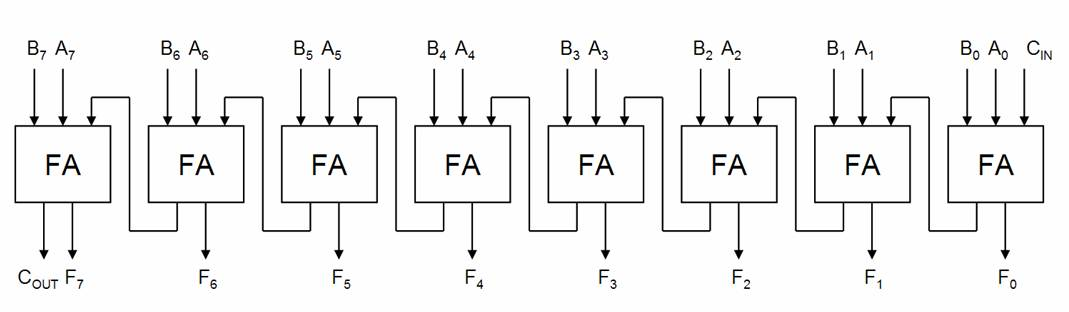
\includegraphics[width=0.9\linewidth]{rca.jpg}
  \caption{A ripple carry adder.}
  \label{fig:etikett}
\end{figure}

The ALU includes a comparator unit which is used to check whether the operands are equal or not. You can implement it by using the structural or dataflow style of VHDL. We decided to do the dataflow implementation because we thought it would be easier and that it would result in a more clean code. In order to check whether the operands are not equal we performed a bitwise XOR on the operands and OR:ed the results. This was used as the resulting NEQ signal. The EQ signal was simply an inversion of the NEQ signal. 

If we were to do this in structural VHDL we would have to create a component which cheked if two certain bits were not equal. We would then have to create eight such components. The input as a whole is equal if all 8 bits are equal, otherwise not.

The operation A minus B is performed by converting B to its 2-complement and then adding it with A. By passing B through 8 XOR gates, each having SUB as its second input, we can form B:s 1-complement when subtracting. We connect SUB to carry-in to form the 2-complement.

\begin{figure}[h!]
  \centering
  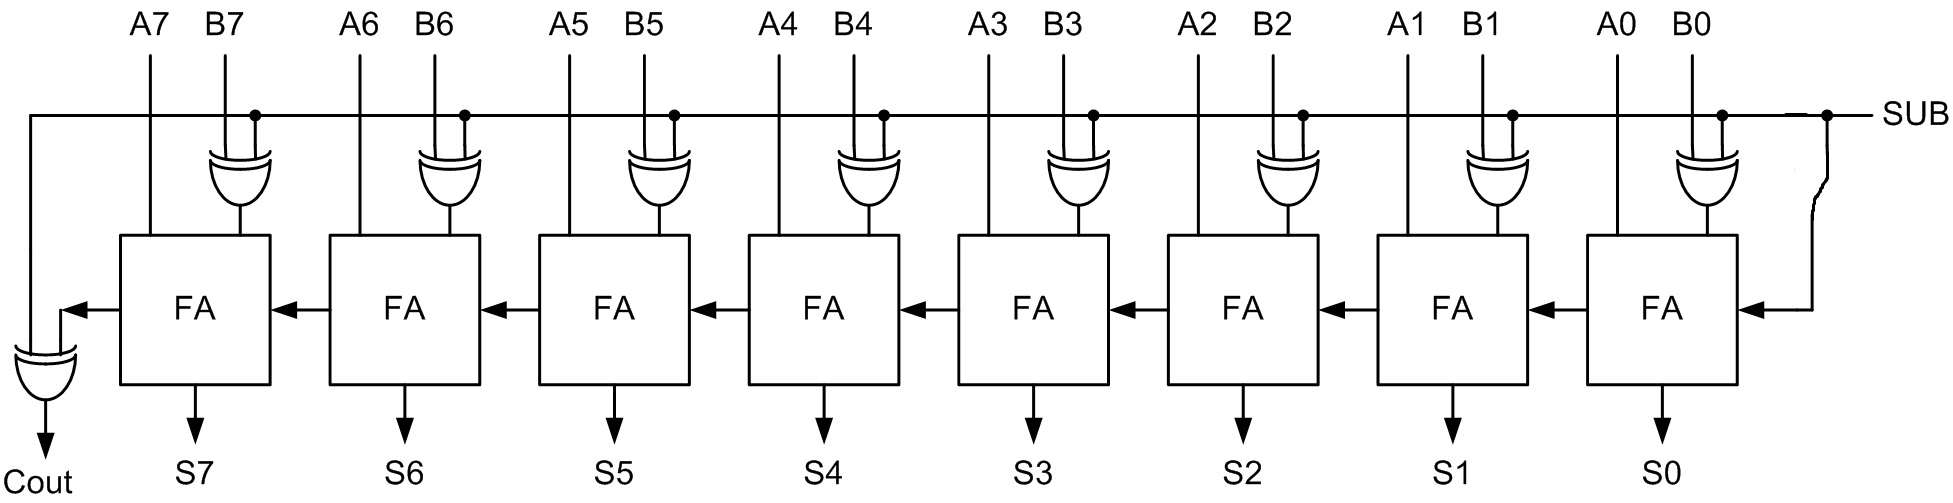
\includegraphics[width=0.90\linewidth]{subtractionlogic.jpg}
  \caption{Logic for performing subtraction with an adder.}
  \label{fig:etikett}
\end{figure}

One thing that we learned was that in VHDL the entity names in a project have to be unique for all references to work properly. 

We also learnt why the critical path for an n-bit RCA is $2n+1$ gates. For every full adder the carry-out depth depends on the inputs ($3$ gates deep) and the carry-in ($2 + $previous depth). The depth is the maximum of these. For the first the depth becomes $3$, for the second $5$ and so on. In other words, for the first adder the inputs are the fartherest away, but for the following it is the carry-in instead. 

\newpage
\subsection{Top-level Design}
\textbf{Registers}\\
We made a generic implementation of a register by letting a variable hold an integer representing the number of bits the register is able to hold. The vectors for in- and output to the register are adjusted after this variable. We implemented our register using behavioral VHDL,i.e using a process statement, since that seemed to result in the simplest and cleanest code. Another reason for using a process statement is that we know that assigning signals values in a process statement result in flip-flops when the code is synthesized.

\textbf{Memory}\\
We also made our implementation of the memory generic. We have two integer variables, one describing the number of address bits ($addr\_width$) and one describing the number of bits each memory location can hold ($data\_width$). The number of bits in the input signals for address and data are adjusted after these variables. The memory itself is an array of a type which we specified. The number of entries in this type of array is $2^{addr\_width}$ and the size of each entry is $data\_width$. The read operation is asynchronous and the write operation is synchronous.

\begin{figure}[h!]
  \centering
  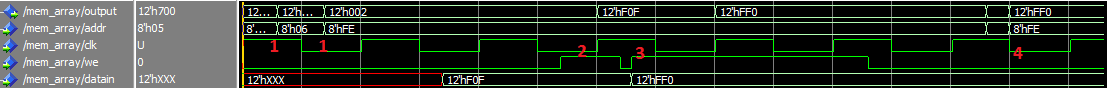
\includegraphics[width=\linewidth]{inst_mem_2.PNG}
  \caption{The operation of the memory.}
  \label{fig:memory}
\end{figure}

In figure \ref{fig:memory} interesting things happen at the red numbers.

\begin{enumerate}
	\item The read is asynchronous, so the output is changed directly after the address is changed.
	\item The write is synchronous, so the write does not happen until the positive edge.
	\item When the input is changed, no write happens at the negative edge.
	\item If we changed the address to something else, and then change back, the value previously written is still saved.
\end{enumerate}

\textbf{Bus}\\
The bus was implemented with a mux. The 4 indata signals each had 8 bits. Bit 0 from each goes to a 4 to 1 mux, bit 1 from each to another mux and so on, i.e. the signals were muxed bitwise. The muxes are inferred by the tools since we used a \textit{WITH SELECT} statement. The mux select signal was created from a one-hot representation of the 4 control signals. Based on which bit was set, the corresponding mux select signal was created. If more than 1 bit are set, the bus error signal is set.

We used a multiplexer for the bus since if 2 or more control signals are set, the bus will not take an undefined value, as opossed to a tri-state version. If 0 or more than 1 control signals are set, we put 0's on the bus since we will not read from it anyway if that is the case.

\textbf{Datapath}\\
The last step was to connect all components of the datapath as described by figure \ref{fig:datapath}. In the datapath entity we had signals with the same names as on that figure (made it easier to code if the names were the same). We then instatiated all components and connected them according to the figure. Some components, such as the registers, have different datawidths in different places. But since they were generic it was easy to have multiple versions.

\begin{figure}[h!]
  \centering
  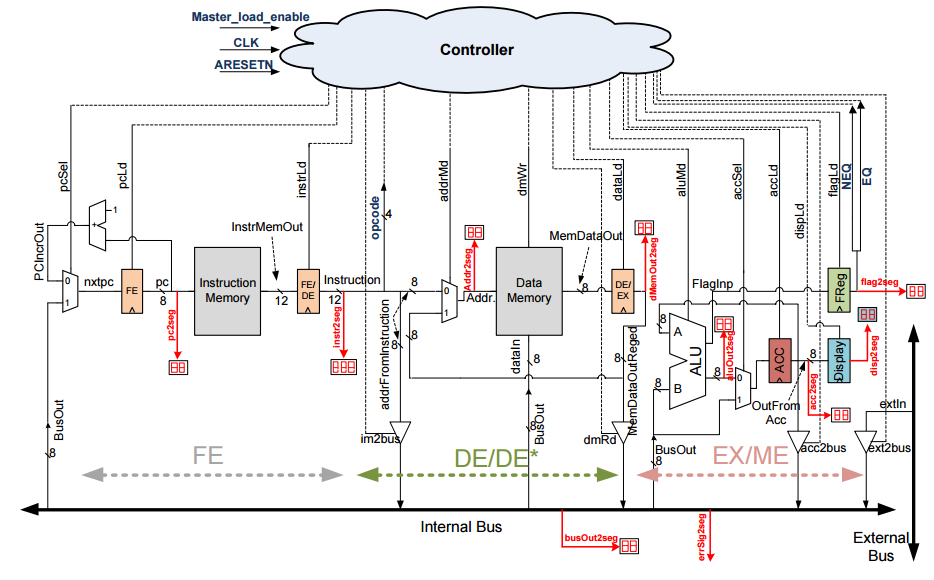
\includegraphics[width=\linewidth]{datapath.png}
  \caption{The datapath of the processor.}
  \label{fig:datapath}
\end{figure} 

\newpage

\subsection{Controller}

\textbf{The FSM} \\
We chose to design our controller as a Mealy FSM. We did this in order to reduce the amount of states (fewer flip-flops). If we would've chosen a Moore design we would roughly need one state for each combination of opcode and stage, although we would be able to minimize it to some extent. Fewer states means that we only have to keep track of five states, namely the stages (FE,DE,DE*,EX,ME), and hence the resulting VHDL code as well as the circuit itself becomes simpler. The statements for assigning the output signals a value are rather long. This would however be the case no matter which design we chose. If we had chosen a Moore design each row in these statements would represent a state and hence the code would be equally long. 

\begin{figure}[h!]
  \centering
  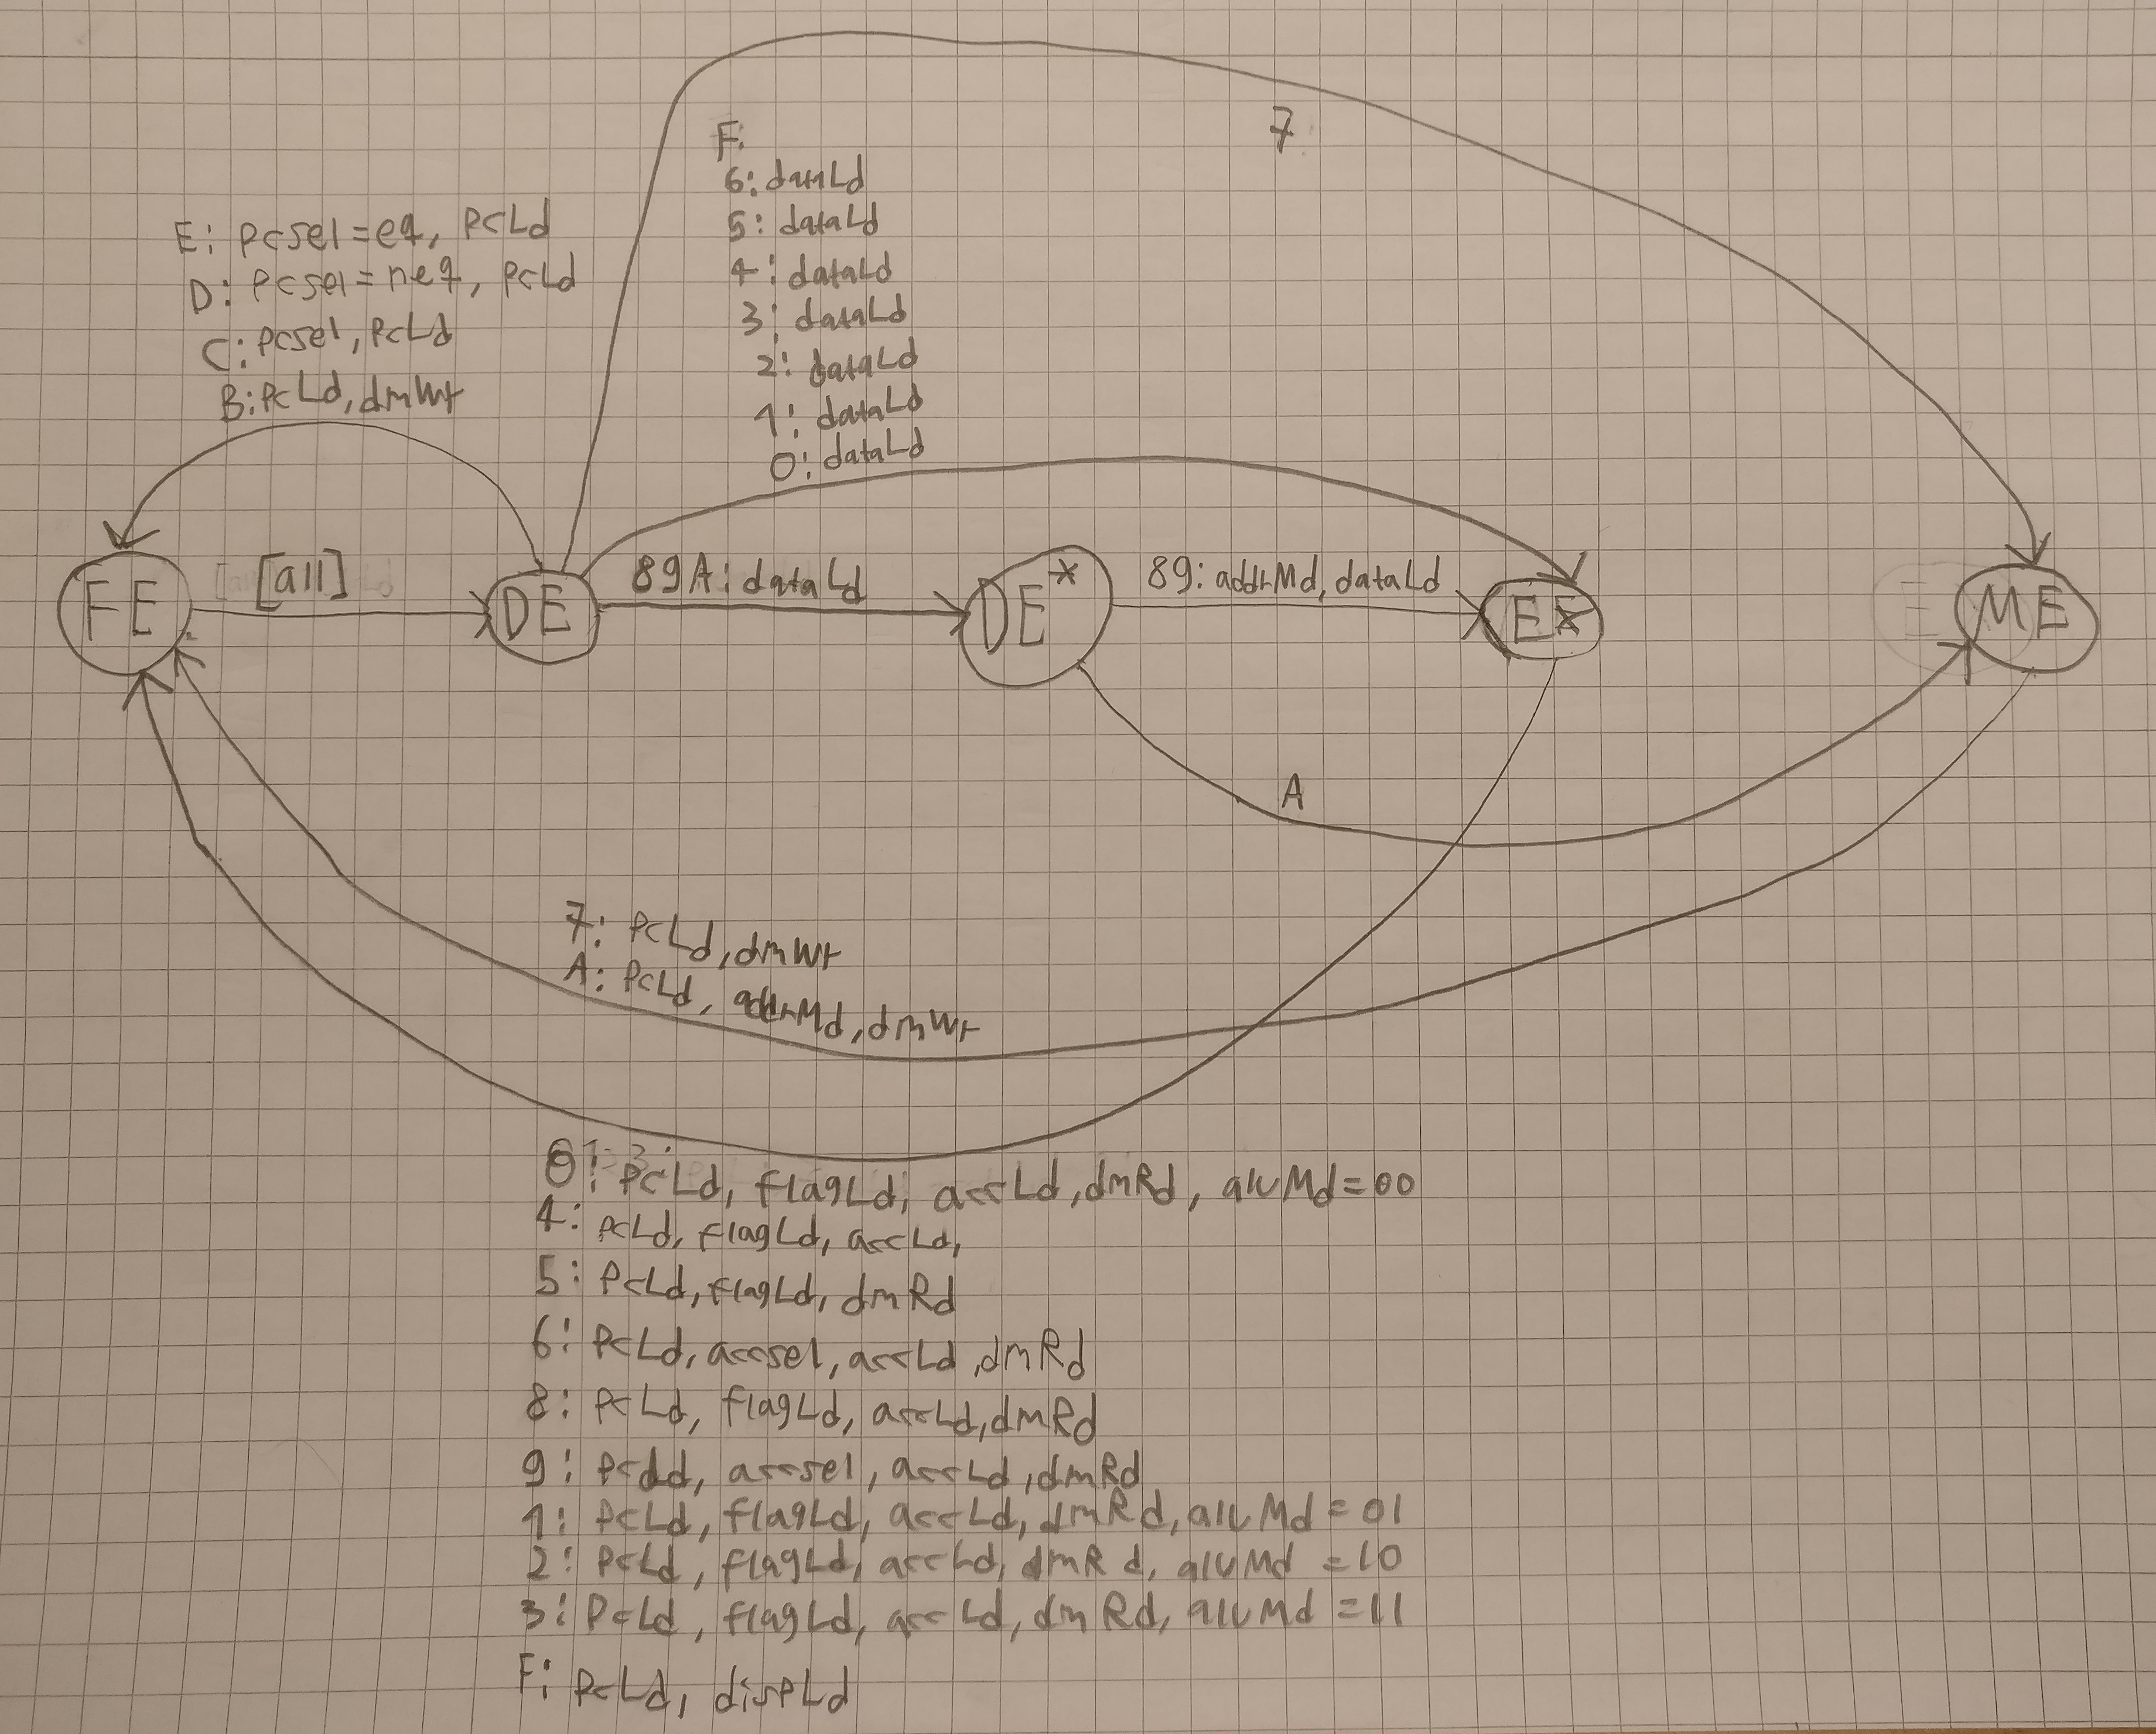
\includegraphics[width=0.7\linewidth]{states.jpg}
  \caption{The state diagram.}
  \label{fig:etikett}
\end{figure}

\textbf{Testing} \\
When we first ran the testbench we noticed a problem. The contents of the data memory did not match the specifications of what it should contain after running the testbench. We started troubleshooting and found three problems.

\begin{enumerate}
  \item We found that our EQ and NEQ signals to the controller weren't assigned at all. We fixed this but the problem remained.
  \item We continued to troubleshoot the controller by examining the waveform diagram of the controller and datapath when running the testbench. While doing this we noticed that after about 500ns the opcodes didn't match the instructions that should be executed. It turned out that the \textit{dmRd} signal didn't have the correct value when the AND instruction was executed. In the processors specification document this signal was a "don't care" for this opcode when it really should've been set to 1, so we changed it. A few days after writing the code we checked the processors specification document and noticed that this had been changed there as well. We assume that this simply was a mistake. 
  \item The instruction for the jump statement was placed at memory location 256 (index starts from 0). This meant that when we jumped to memory location 255 a \textit{NOOP} instruction was executed, the PC overflowed and then the program started from the beginning. We corrected this by moving the contents of memory location 256 to memory location 255. After this the testbench ran successfully.  
\end{enumerate}

In figure \ref{fig:waves_instr} we see the waveform diagram of instructions 1 to 3 in the test program being executed. If you compare the diagram with the processors specification document it's clear that the signals have the correct value at the correct time. You can also see that it's first after the fetch stage is completed that the opcode changes. This is because the fetch stage has to be completed before the opcode can be sent from the FE/DE register to the controller. 

 \begin{figure}[h!]
  \centering
  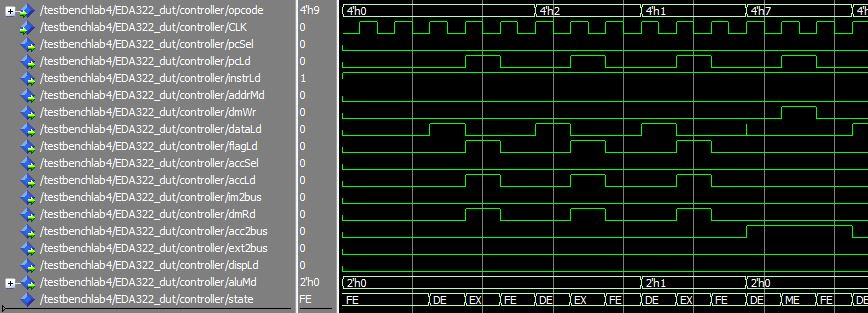
\includegraphics[width=0.75\linewidth]{controller_waves.JPG}
  \caption{The waveform diagram for executing instructions 1 to 3 in the test program.}
  \label{fig:waves_instr}
\end{figure}

Note that when the opcode changes from 1 to 7 in figure \ref{fig:waves_instr} a spike occurs for the signal dataLd. This is an effect of our Mealy design. The output signal only depends on state and input (opcode). Since the stage is DE and the opcode is 1 for a brief moment the \textit{dataLd} signal becomes 1. When the opcode changes to 7 \textit{dataLd} becomes 0. This is not a problem since the spike occurs after the positive edge of the clock. Since everything is synchronous the control signals have corrected themselves before the next positive edge, meaning that no errors will be made. 

\subsection{Processor's Testbench}

The testbench is used to verify the processor's correct operation. By simulating inputs to the processor and examining the outputs you can determine whether an operation was carried out in a correct fashion or not. In practice this is done by writing an assembler program which you load into the memory of the processor. The verification is done by comparing the actual outputs with the expected outputs while running the program on the processor. If any of the outputs take an unexpected value an error has been found.
\\\\
When designing the testbench we initially thought that there were huge issues with the flag register. We got no output to the \textit{flag2seg} signal which indicated that something was wrong with the flag register. This seemed a little bit odd however, since the flag register had worked just fine previously. When checking the VHDL code for the processor it turned out that we'd forgotten to connect the \textit{flag2seg} signal to the flag register. After connecting this our testbench ran successfully. 

\textbf{How the testbench works}
\begin{itemize}
  \item \underline{Generating input.} The input to the processor are the control signlas (\textit{externalIn, clk, master\_load\_enable} and \textit{aresetn}) and the instruction and data memory files. The control signals are assigned values, some periodically,  in the architecture of the testbench. The memory content is read when the memory entities are instantiated. Based on the memory content different output is expected, hence we consider those files an input from the testbench.
  \item \underline{Reading expected outputs.} The expected output values are read from text files into five different arrays, one for each output signals to check. The reading is done inside a process in the testbench architecture. For each file, while it has not reached the end, read the current line. That line is parsed as an 8-bit vector and is stored in the array at the current index. The index is incremented and the same procedure is repeated.
  \item \underline{Comparing outputs and expected outputs.} The output signals of interest have one process each, sensitive to the signal. When that signal changes the process is triggered and its value is compared to its expected value in the array by using asserts. If they are equal, the index for that array is incremented. Otherwise the testbench stops and reports the error. The output signals that are checked are \textit{DataMemOut, flag2seg, pc2seg, acc2seg} and \textit{disp2seg}.
\end{itemize}

\subsection{ChAcc on Nexys 3 board \emph{(Optional)}}
(max: 2 pages)
\\\\
Describe how you verified the correctness of your FPGA implementation. Note that the code that is executed on the implementation is the same code used for testing in Lab 5. You should compare sequences of values on various signals observed on the seven-segment displays to values seen in Modelsim simulation of the design. Please include in the report the sequence of program counter (PC) and display register values you observed during a successful execution on the FPGA. 

\subsection{Performance, Area and Power Analysis \emph{(Optional)}}
(max: 2 pages)
\\\\
To be announced in the Lab7PM.

\newpage
\section{Analysis}

After completing lab 2 to 5 we have a processor which can perform some basic operations. The processor consists of an ALU, registers, memories, muxes, a bus and a controller. Through careful testing and debugging we have verified that each component works as intended, both individually and together. We used waveforms to test the components and a testbench we designed ourselves to test the processor as a whole.

We've made two projects for each of our labs, one using an ALU based on an RCA and one based on a CLA. Although we haven't been able to notice any difference in performance (which we didn't expect to be able to) it's been interesting to see both implementations and how they accomplish the same task. Since the critical path of the CLA is shorter the clock frequency can be increased and the performance enhanced.
 
When testing our controller in lab 4 we had some issues. In order to solve this we needed to use waveforms to check what instructions were being executed as well as if the correct state and control signals were set. By examining the waveforms we were able to track the error to a certain control signal which wasn't set when it should've been. This gave us valuable experience in how to use simulations and waveforms to debug errors.

It was a good learning experience to design the controller as an FSM. Previously we had only designed smaller circuits for the purpose of learning how to do it, and not for use in practice. Designing an FSM for use in practice gave use a better understanding of the characteristics of a mealy FSM compared to a moore FSM (number of states and timing).

The hardware and the testbench have been described in VHDL. We have gained experience in this and also seen the difference between programming and describing hardware in code. Throughout this lab series we have kept in mind to write the VHDL in such a way that no unwnated  hardware (e.g. latches) is synthesized. This was new to us compared to programming, where you can write more freely.

We realize that if the goal was to design an ASIC much more work would be needed. For example we would need to describe the placement of the components on the chip. And if we were to make some errors (which we have done) it would cost both money and time.

% Appendix
\newpage
\begin{appendix}

\section{Appendix}
(max: 4 pages)
\\\\
In the appendix, you can include extra figures or tables that don't fit in the main body of the lab report. 

\end{appendix}

\end{document}
